\documentclass[11pt]{article}
\usepackage[left=0.65in,right=0.65in,top=0.7in,bottom=0.8in]{geometry}

\usepackage{amsmath,amssymb}
\usepackage{iftex}
\usepackage{tikz-cd}
\usepackage{titlesec}
\usepackage{graphicx}
\graphicspath{{../}{./}}
\usepackage{xcolor}
\usepackage{float}
\ifPDFTeX
\usepackage[T1]{fontenc}
\usepackage[utf8]{inputenc}
\usepackage[sfdefault]{carlito}
\renewcommand{\familydefault}{\sfdefault}
\else
\usepackage{fontspec}
\IfFontExistsTF{Calibri}
  {\setmainfont{Calibri}}
  {\setmainfont{Carlito}}
\fi

\usepackage[backend=biber,style=numeric,sorting=none]{biblatex}

\addbibresource{references.bib}

\setlength{\parindent}{1em}
\setlength{\parskip}{0pt}
\raggedbottom
\setlength{\emergencystretch}{2em}
\titlespacing*{\section}{0pt}{0.7\baselineskip}{0.4\baselineskip}
\titlespacing*{\subsection}{0pt}{0.55\baselineskip}{0.3\baselineskip}
\titlespacing*{\paragraph}{0pt}{0.35\baselineskip}{0.5em}

\newcommand{\AIon}{\color{blue!65!black}}
\newcommand{\Reviewed}{\color{black}}
\newcommand{\supervisornote}[1]{\par\begingroup\color{gray}\small #1\par\endgroup}
\newcommand{\supervisorgraphic}[2][]{%
  \begin{tikzpicture}
    \node[inner sep=0, outer sep=0] (img) {\includegraphics[#1]{#2}};
    \fill[white, opacity=0.45] (img.south west) rectangle (img.north east);
    \draw[gray!70, line width=0.6pt] (img.south west) rectangle (img.north east);
    \node[anchor=north east, xshift=-4pt, yshift=-4pt, fill=gray!80, text=white, rounded corners=2pt, inner xsep=5pt, inner ysep=2pt, font=\sffamily\bfseries\scriptsize] at (img.north east) {Supervisor only};
  \end{tikzpicture}%
}

\title{Toward Testing the One-Vote-Veto Hypothesis in Overall IEQ Satisfaction in Belgian Classrooms}
\author{}
\date{\today}

\begin{document}

\AIon

\maketitle
\begin{abstract}

\end{abstract}
\vspace{0.2\baselineskip}

\section{Introduction}

\subsection{Context and Problem Definition}

Indoor environmental quality (IEQ) describes several conditions in a room, mainly thermal comfort, air quality, lighting, and acoustics. In classrooms, these conditions can affect students' comfort, engagement, and learning \cite{carton2023iaqvec,sadick2017,carton2023primary}. This paper focuses on overall IEQ satisfaction: how students judge the classroom environment as a whole, instead of looking at only one domain such as temperature or air quality \cite{wong2008,heinzerling2013,frontczak2012}.

The study uses the open Belgian classroom dataset, which includes repeated satisfaction votes from primary, secondary, and higher-education classrooms, together with synchronized environmental and contextual data \cite{carton2026dataset}. This makes it possible to model overall IEQ satisfaction as a combined, multi-domain outcome.

\subsection{Literature Review and Research Gap}

Research on IEQ does not support treating overall satisfaction as a thermal-only outcome. Office studies and IEQ reviews show that overall satisfaction is shaped by several domains, including thermal comfort, air quality, acoustics, visual conditions, spatial factors, and their interactions \cite{wong2008,frontczak2012,heinzerling2013,zhao2023}. Recent modelling work also shows that simple fixed weights may miss nonlinear and context-dependent relationships, and that IEQ models need validation on field data rather than only fitting one dataset \cite{tang2022,zhao2023}.

Classrooms are a weaker part of this evidence base. Much of the multi-domain IEQ evidence comes from offices, while students have limited control over the indoor environment and may not respond like adults. School studies and reviews report that standard comfort models often predict student responses poorly, and call for more classroom-specific and longitudinal modelling work \cite{teli2012,lala2022children,miao2024students}. A recent review of subjective air-quality assessment also shows a broader methodological problem: studies differ in survey scales, study design, sample size, and modelling methods, which makes comparison and reuse difficult \cite{carton2026review}.

The Belgian classroom dataset helps address these gaps because it links repeated overall and domain satisfaction votes with environmental, personal, and contextual variables in primary, secondary, and university classrooms \cite{carton2026dataset}. This paper uses that dataset to test how well individual overall IEQ satisfaction can be predicted from the variables available before or during a classroom session. The contribution is a classroom-specific benchmark with transparent preprocessing, comparable metrics, and feature-importance analysis. It shows what can be predicted, which variables appear useful, and where current models remain uncertain.

\subsection{Research Questions}

\begin{enumerate}
    \item \textbf{RQ1: To what extent can overall classroom IEQ satisfaction be predicted from environmental, contextual, and building-related variables?}

    \item \textbf{RQ2: Which predictors contribute most to the prediction of overall IEQ satisfaction?}

    \item \textbf{RQ3: How can transfer learning be used to improve the generalization of classroom IEQ satisfaction models across different educational settings?}
\end{enumerate}

\subsection{Contribution}

\begin{itemize}
    \item A classroom-specific benchmark for predicting three-class overall IEQ satisfaction from environmental and contextual variables, with transparent preprocessing and comparable metrics across five model families (RQ1, RQ2).
    \item A transfer-learning analysis testing how well models trained on one educational setting generalize to others (RQ3).
    \item A feature-importance analysis identifying which variables are most useful for predicting overall IEQ satisfaction in classrooms.
    \item A practical reference for school operators: the models could support a classroom dashboard that flags lessons or rooms with a higher risk of poor IEQ, helping to decide when to check ventilation, temperature, lighting, or noise conditions.
    \item An argument for holistic building control: unlike four independent domain models, an overall IEQ model can capture cross-domain trade-offs. A control system using it could, for example, open blinds for passive solar heating while accepting a minor reduction in visual comfort---optimizing occupant satisfaction relative to energy cost rather than treating each domain in isolation.
\end{itemize}

{\Reviewed
\section{Dataset Description}

The source material is the open Belgian classroom dataset with 6{,}834 satisfaction assessments from 321 occupants across 11 classrooms in three educational settings: primary school, secondary school, and a university test lecture room \cite{carton2026dataset}. In this study, the combined dataset is used as the empirical basis for the overall IEQ prediction.

The main target is overall IEQ satisfaction on the original five-point scale. The dataset also includes synchronized environmental measurements such as air temperature, relative humidity, CO$_2$, illuminance, and LAeq, together with contextual and occupant variables including age, gender, clothing, seat position, classroom type, and timing information.

This draft uses the dataset description as the empirical starting point for the IEQ article. Any later feature-selection refinements, benchmark analyses, and interpretation will therefore be developed specifically for the overall IEQ paper after the next round of model runs is completed.}

\supervisornote{Supervisor note: cases 1 and 2 (secondary and primary schools) were collected during the COVID period, so the dataset may reflect classroom conditions under stronger-than-usual ventilation. This is especially relevant for CO$_2$, because more intensive window opening may have narrowed the observed range compared with ordinary classroom operation. A reviewer may raise this point, so it should later be acknowledged explicitly as a study limitation rather than treated as a minor side issue.

The following graphs are here only to help understanding the dataset.}

\begin{figure}[H]
    \centering
    \supervisorgraphic[width=0.88\textwidth]{04_Figures/both_papers/fig_01_raw_dataset_column_completeness.pdf}
    \caption{Supervisor-only supporting figure: raw dataset column completeness across the shared classroom dataset.}
    \vspace{-0.40\baselineskip}
\end{figure}

\begin{figure}[H]
    \centering
    \supervisorgraphic[width=0.88\textwidth]{04_Figures/both_papers/fig_04_satisfaction_vote_distribution.pdf}
    \caption{Supervisor-only supporting figure: satisfaction vote distributions across the overall IEQ target and the four domain targets on the original five-class scale.}
    \vspace{-0.40\baselineskip}
\end{figure}

\begin{figure}[H]
    \centering
    \supervisorgraphic[width=0.88\textwidth]{04_Figures/both_papers/fig_04b_unified_satisfaction_category_distribution.pdf}
    \caption{Supervisor-only supporting figure: unified satisfaction-category distributions across the shared target set.}
    \vspace{-0.40\baselineskip}
\end{figure}

\begin{figure}[H]
    \centering
    \supervisorgraphic[width=0.995\textwidth]{04_Figures/ieq_paper/fig_05_ieq_environmental_feature_boxplots.pdf}
    \caption{Supervisor-only supporting figure: environmental feature boxplots for the IEQ paper variables.}
\end{figure}

{\Reviewed
\subsection{Data Cleaning and Imputation}

Before imputation, the predictor set was defined to cover the main IEQ domains in the dataset while retaining a limited set of occupant and situational descriptors. The retained variables and their completeness are summarized in Figure~\ref{fig:ieq-feature-completeness}. Trace and grouping identifiers were excluded to reduce identity- or classroom-specific leakage and to keep the models focused on interpretable predictors.}

\begin{figure}[H]
    \centering
    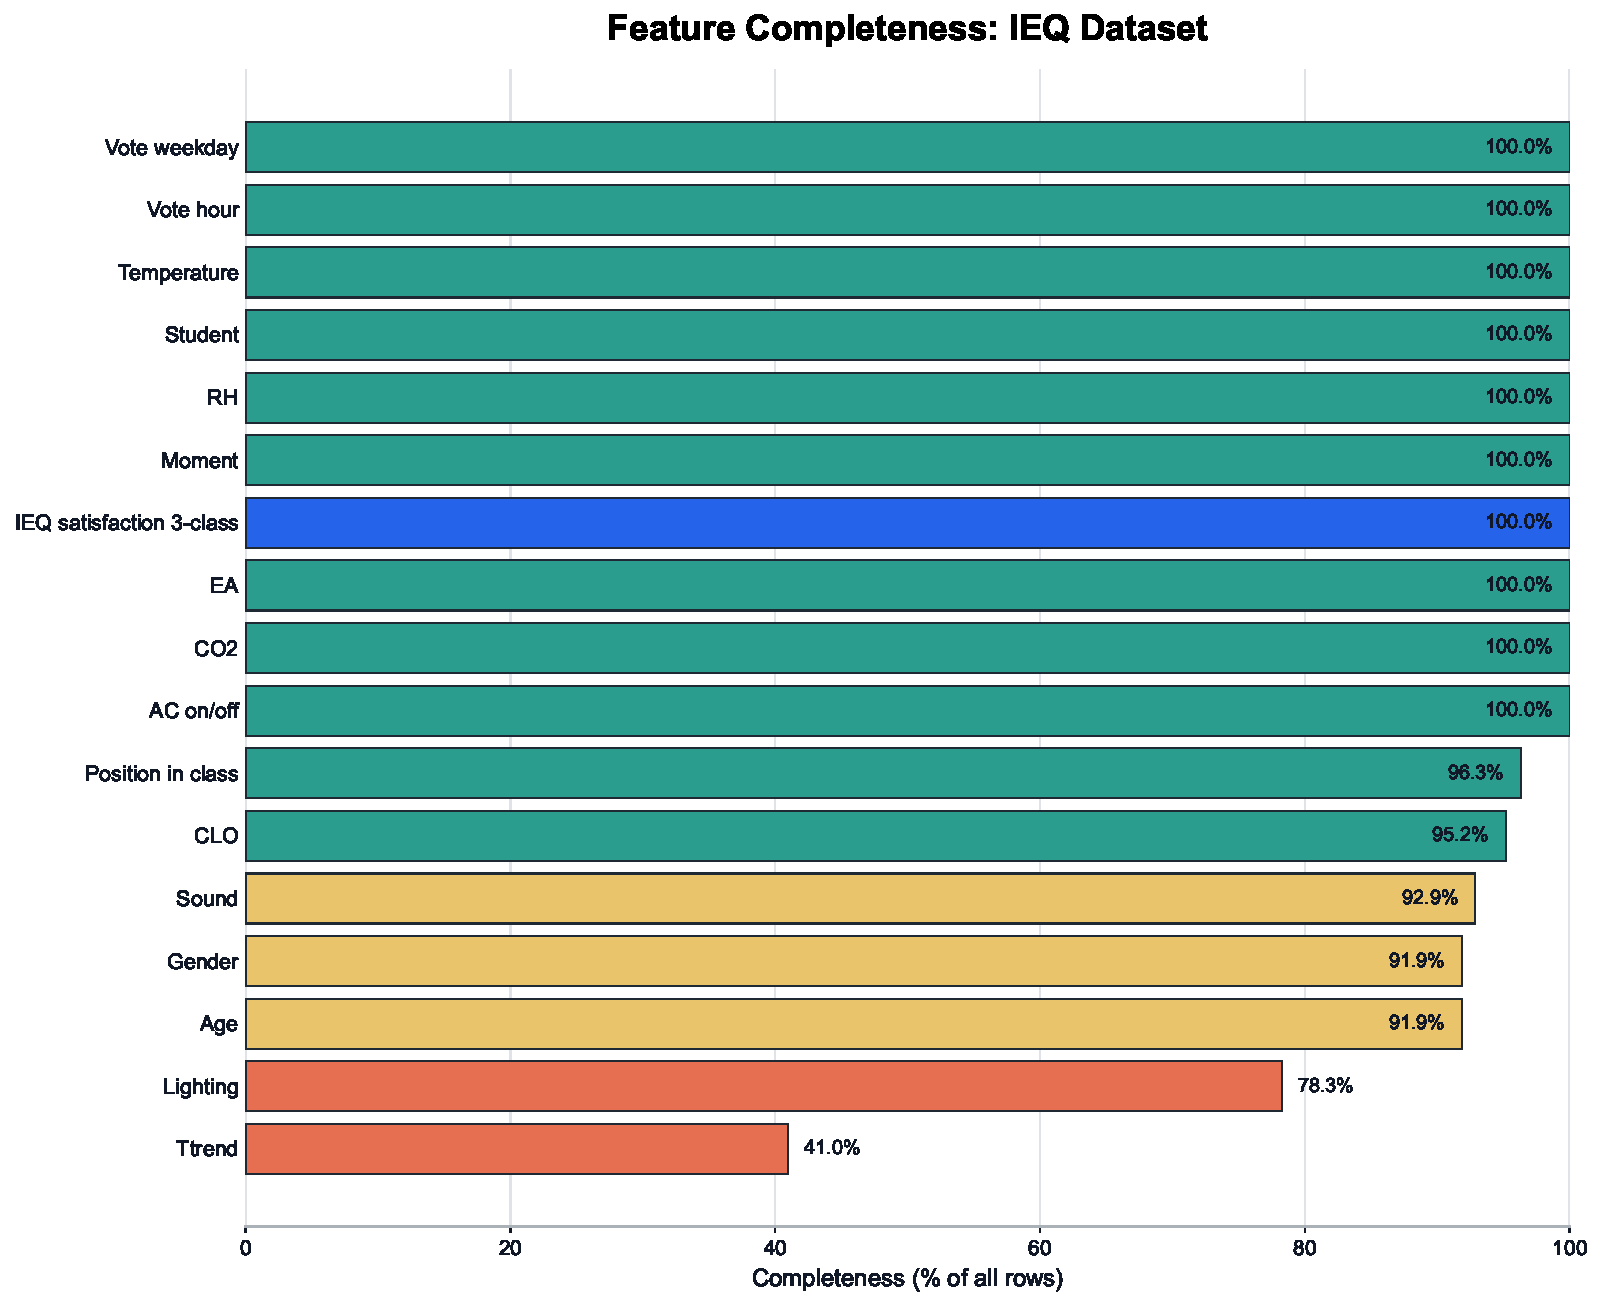
\includegraphics[width=0.82\textwidth]{04_Figures/ieq_paper/fig_03_ieq_feature_completeness.pdf}
    \caption{Feature completeness for the variables currently retained in the IEQ paper.}
    \label{fig:ieq-feature-completeness}
    \vspace{-0.35\baselineskip}
\end{figure}

{\Reviewed
Missing values were filled using fixed, reproducible rules. Missing classroom position was set to Middle. Clothing insulation (CLO) was imputed by the median within each Group, with the global dataset median used as fallback. In the survey and dataset documentation, clothing is recorded as either a simple three-level category (light, neutral, warm) or a more detailed clothing description, not as a directly measured insulation value. Here, the simple categories were mapped to approximate clo values of 0.44, 0.64, and 0.81 based on standard clothing-insulation tables; these values should therefore be interpreted as representative approximations rather than observed measurements \cite{carton2026dataset,ashrae2023standard55,pythermalcomfortclothing2025}. Temperature trend, sound level, and lighting were imputed by the median within Group + Subgroup, then by Group, and finally by the global median as a fallbacks. Age was first inferred from other records with the same Occupant ID using that occupant's median reported age; if no age was available for that ID, the fallback sequence was the median within Group + student-status, then Group, then the global median. Gender was first copied from other records with the same Occupant ID; if no gender was available for that ID, it was assigned by a seeded random draw from the gender distribution within the same Group, with the overall dataset distribution used as fallback. The original five-category overall IEQ scale (1 = very dissatisfied, 2 = dissatisfied, 3 = ok, 4 = satisfied, 5 = very satisfied) was collapsed into three classes for modeling purposes, with categories 1 and 2 merged as dissatisfied, category 3 retained as neutral, and categories 4 and 5 merged as satisfied. The distributions on both scales are shown in Figure~\ref{fig:overall-ieq-distribution}.}



\begin{figure}[H]
    \centering
    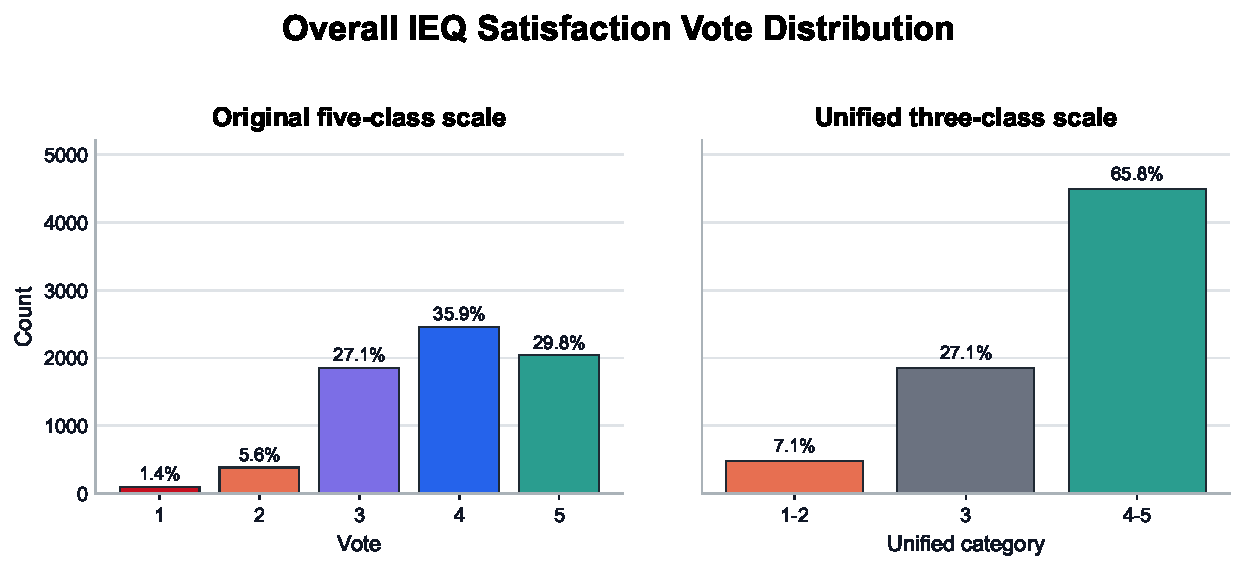
\includegraphics[width=0.88\textwidth]{04_Figures/ieq_paper/fig_overall_ieq_satisfaction_vote_distribution_original_unified.pdf}
    \caption{Original and unified overall IEQ satisfaction vote distributions in the current dataset.}
    \label{fig:overall-ieq-distribution}
\end{figure}

\supervisornote{Supervisor note: the following supporting figures are intentionally greyed out in the draft to show that they are included only for discussion, orientation, and easier interpretation. They are not yet intended as part of the core article narrative.}



\clearpage
\section{Analysis}
{\Reviewed
\subsection{Modeling Setup}

The cleaned dataset was used for ML modelling three-class overall IEQ satisfaction label (dissatisfied, neutral, satisfied). All models were evaluated with five-fold cross-validation using the same folds for fair comparison. The first benchmark stage compared Logistic Regression, Gradient Boosting, ANN/MLP, Random Forest, and Extra Trees. Because the class distribution is imbalanced toward the satisfied class, macro F1 (a score that gives equal importance to all three classes) was used as the main model-selection metric, while raw accuracy, balanced accuracy, and ordinal mean absolute error (MAE) were retained as complementary diagnostics.

\subsection{Tuning Workflow}

The analysis was done step by step so the draft shows not only the final result, but also how we got there.
\begin{enumerate}
    \item First, we compared five baseline models on the same feature set.
    \item Next, we tuned the strongest models.
    \item Extra Trees then received an additional tuning round because it performed best.
    \item Finally, we tested several follow-up variants and checked whether the results stayed similar under slightly different settings.
\end{enumerate}}

\section{Results}
{\Reviewed
\subsection{Main Tuned Benchmark}

The tuned comparison identifies Extra Trees as the strongest single model for the all-school IEQ benchmark. Extra Trees was the strongest single model in the main benchmark. Random Forest remains the closest competitor, while the simpler linear baseline and the weaker nonlinear baselines lag clearly behind on macro F1.}

\begin{table}[H]
    \centering
    \small
    \caption{Tuned five-fold cross-validation summary for the current all-school IEQ benchmark.}
    \label{tab:ieq-main-benchmark}
    \begin{tabular}{lccccc}
        \hline
        Model & Accuracy & Bal. acc. & Macro F1 & Weighted F1 & Ordinal MAE \\
        \hline
        Extra Trees & 0.722 & 0.592 & 0.591 & 0.719 & 0.316 \\
        Random Forest & 0.713 & 0.584 & 0.582 & 0.708 & 0.326 \\
        ANN / MLP & 0.698 & 0.495 & 0.517 & 0.676 & 0.345 \\
        Gradient Boosting & 0.692 & 0.446 & 0.464 & 0.635 & 0.356 \\
        Logistic Regression & 0.483 & 0.464 & 0.401 & 0.521 & 0.671 \\
        \hline
    \end{tabular}
\end{table}

{\Reviewed
Extra Trees therefore becomes the current paper-facing reference model. It performs better than the tuned Random Forest on the main benchmark metrics and also improves on the earlier tuned Extra Trees version.}

\begin{figure}[H]
    \centering
    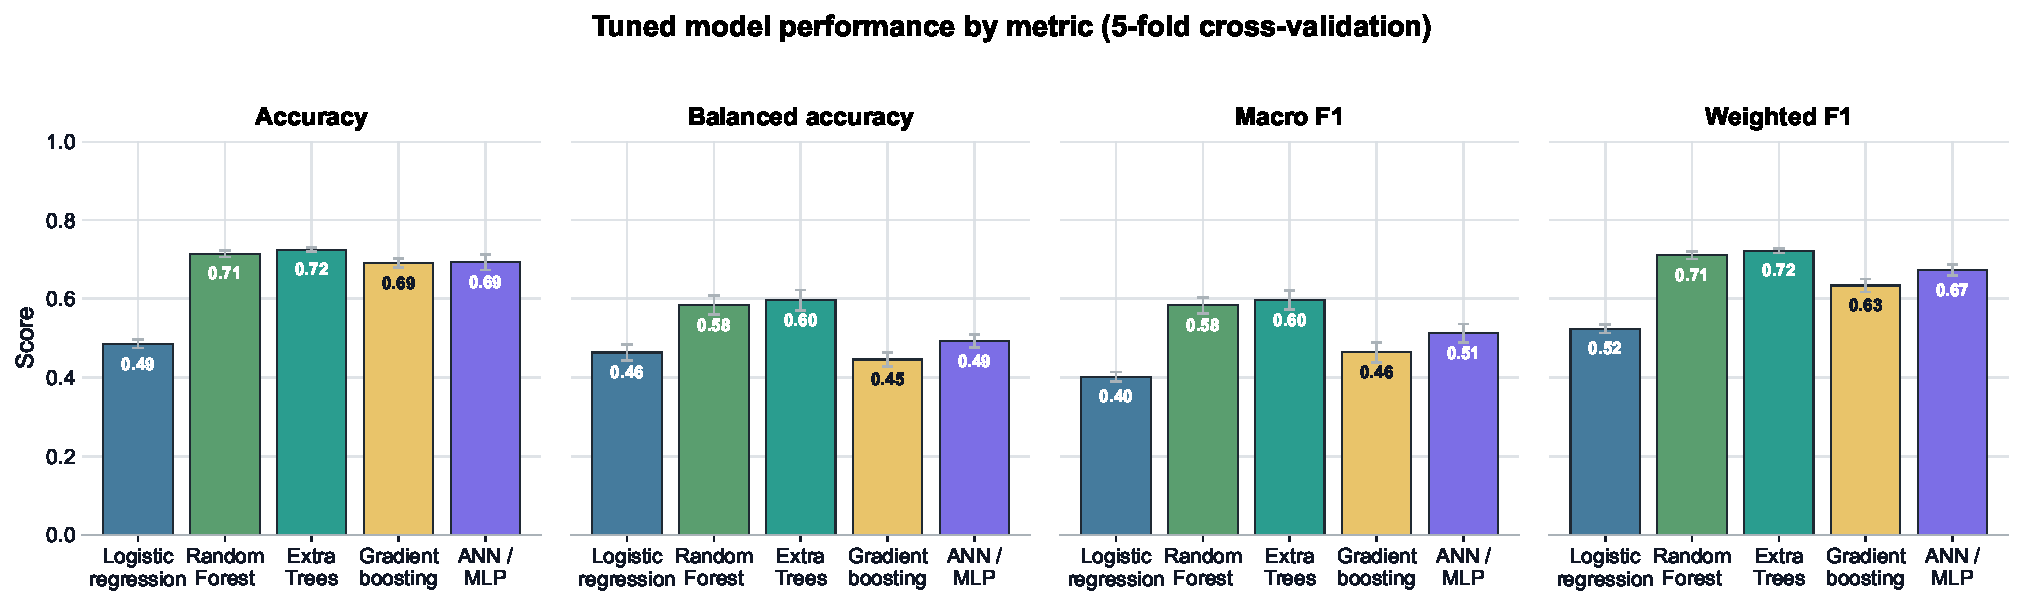
\includegraphics[width=0.88\textwidth]{04_Figures/ieq_paper/tuned_model_comparison_performance.pdf}
    \caption{Performance comparison for the tuned IEQ benchmark models under five-fold cross-validation.}
    \label{fig:ieq-tuned-performance}
\end{figure}

\begin{figure}[H]
    \centering
    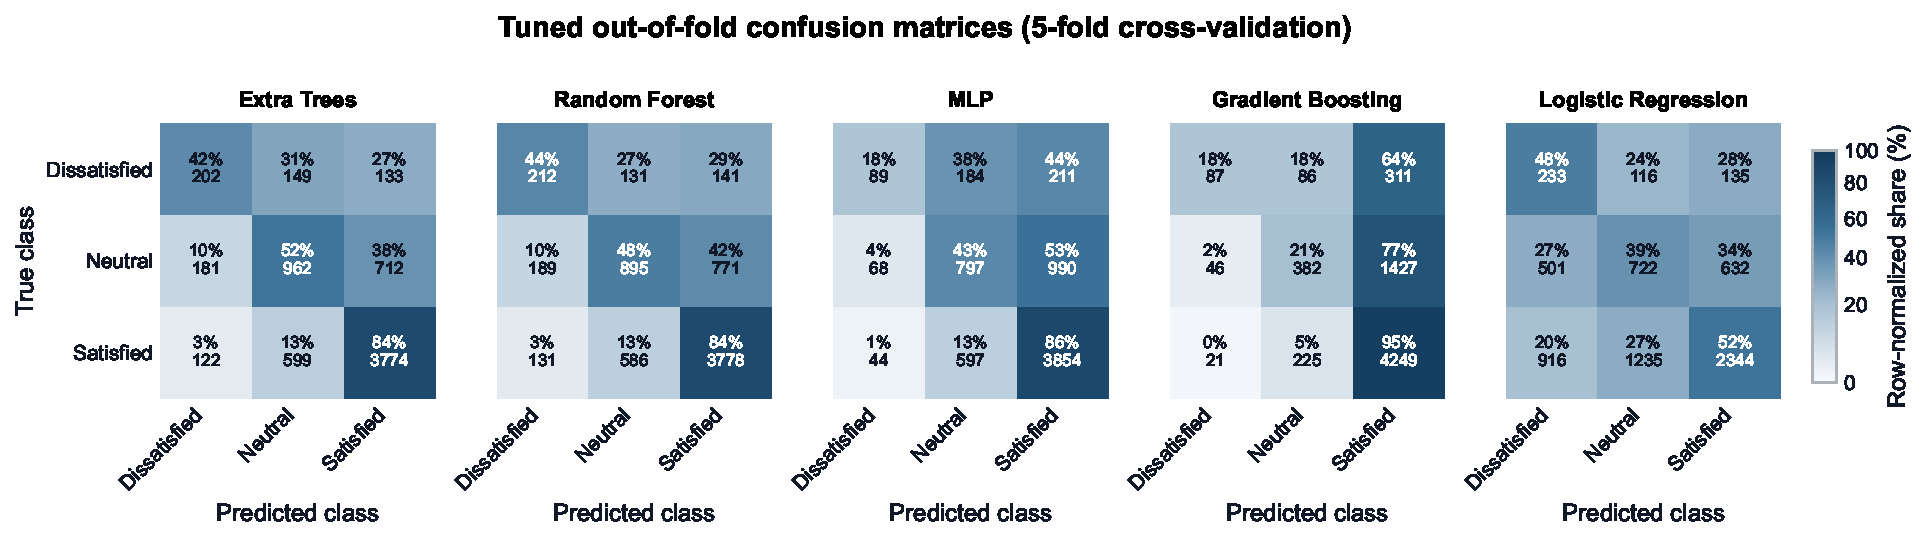
\includegraphics[width=0.93\textwidth]{04_Figures/ieq_paper/tuned_model_comparison_confusion_matrices.pdf}
    \caption{Aggregated confusion matrices for the tuned IEQ benchmark models.}
    \label{fig:ieq-tuned-confusion}
\end{figure}

{\Reviewed
The confusion patterns help explain why macro F1 is a more informative selection metric than raw accuracy in this problem. For the refined Extra Trees model, the satisfied class is recognized strongly, but the model still recovers 42.1\% of dissatisfied votes and 53.0\% of neutral votes. Random Forest behaves similarly but is slightly weaker for the neutral class. Gradient Boosting and ANN/MLP push too many cases into the satisfied class, which inflates apparent accuracy while damaging minority-class performance. Logistic Regression is the clearest baseline showing that simple linear decision boundaries are insufficient for this classroom IEQ target.

\begin{figure}[H]
    \centering
    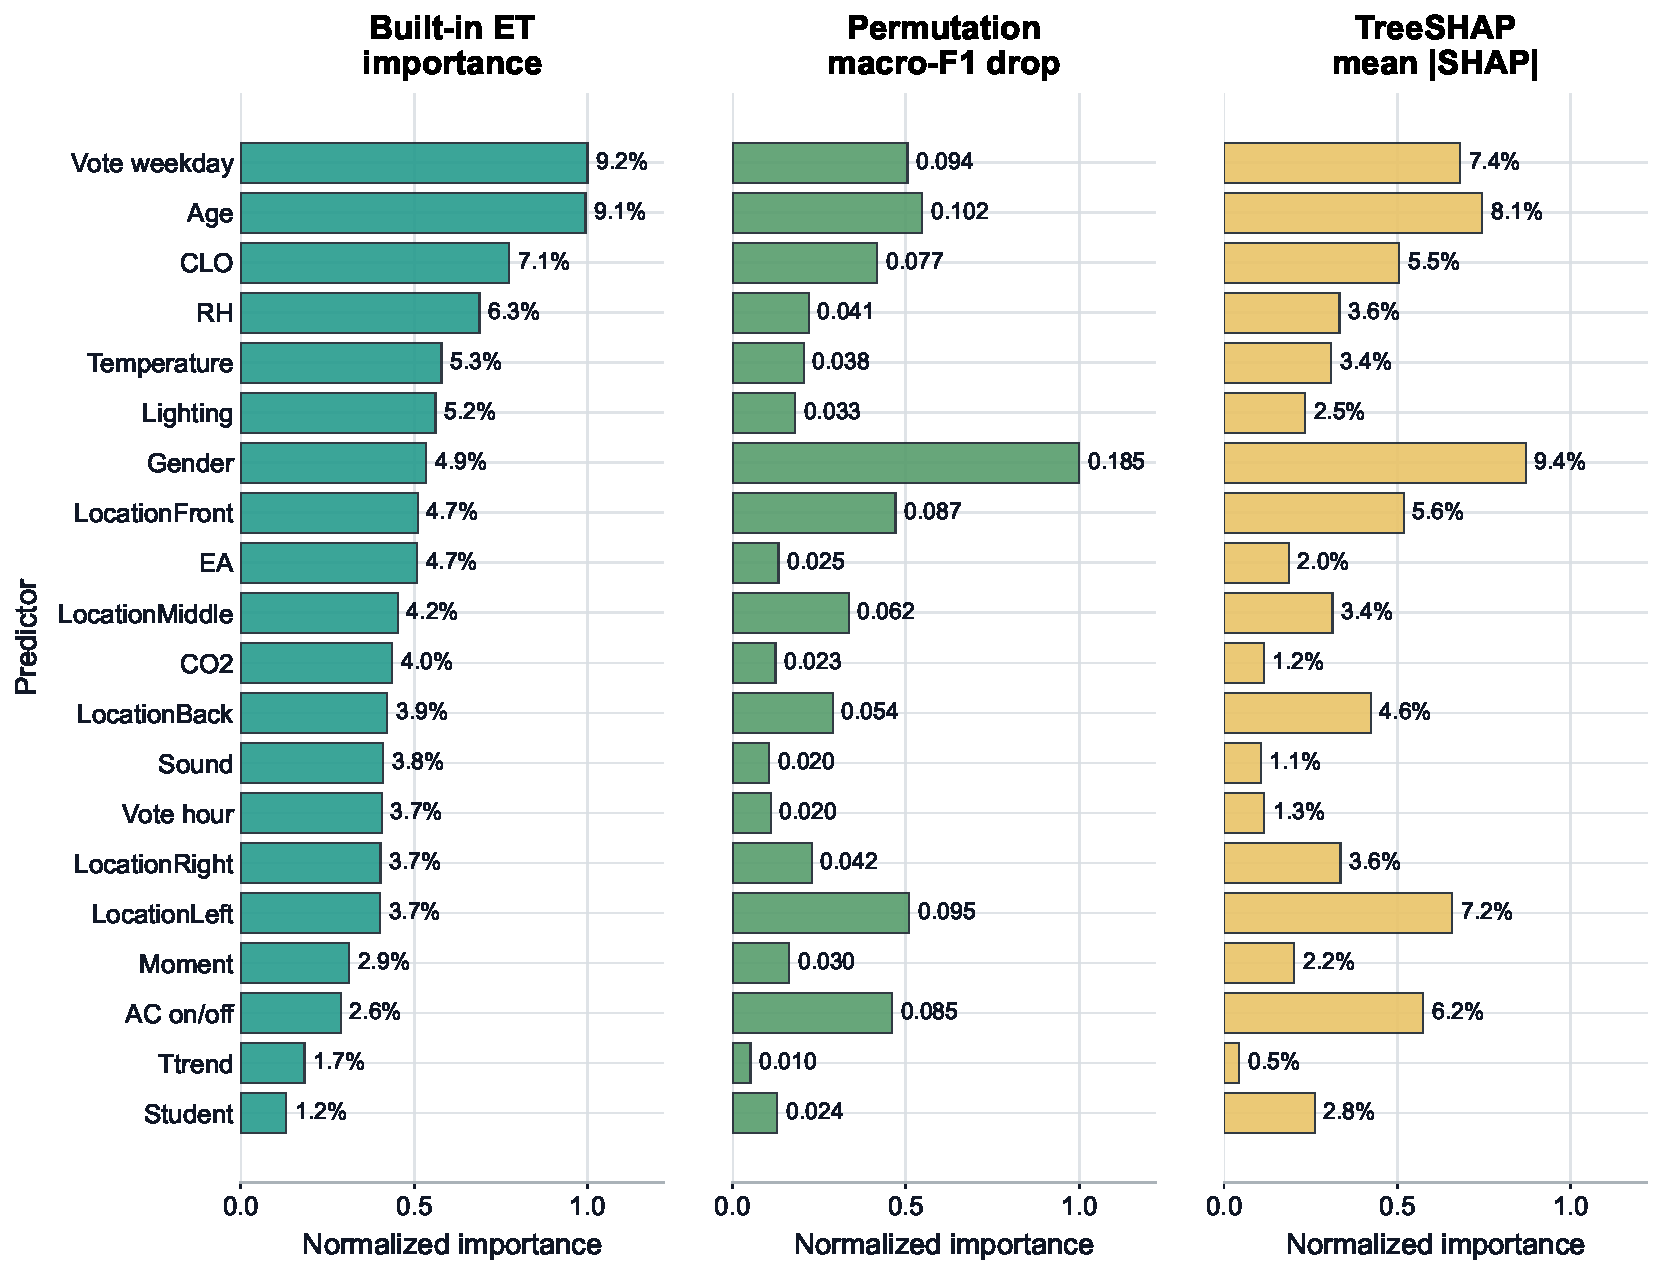
\includegraphics[width=0.98\textwidth]{04_Figures/ieq_paper/final_extra_trees_importance_method_comparison.pdf}
    \caption{Feature-importance comparison for the final Extra Trees IEQ prediction model.}
    \label{fig:ieq-feature-importance}
\end{figure}

The feature-importance results vary drastically depending on the method, model or even hyperparameters used. Therefore, the figure is useful for identifying potentially important predictors, but it should not be read as a definitive causal explanation of overall IEQ satisfaction.

\subsection{Best Hyperparameters}

\begin{table}[H]
    \centering
    \small
    \caption{Best tuned configurations for the main IEQ model families.}
    \label{tab:ieq-best-params}
    \begin{tabular}{p{2.7cm}p{10.6cm}}
        \hline
        Model & Selected hyperparameters \\
        \hline
        Extra Trees & \texttt{n\_estimators=700}, \texttt{criterion=entropy}, \texttt{bootstrap=True}, \texttt{max\_samples=0.9}, \texttt{max\_features=None}, \texttt{max\_depth=20}, \texttt{min\_samples\_leaf=2}, \texttt{min\_samples\_split=10}, \texttt{class\_weight=balanced} \\
        Random Forest & \texttt{n\_estimators=300}, \texttt{max\_depth=20}, \texttt{max\_features=sqrt}, \texttt{min\_samples\_leaf=4}, \texttt{min\_samples\_split=10}, \texttt{class\_weight=balanced} \\
        ANN / MLP & \texttt{hidden\_layer\_sizes=(32,)}, \texttt{activation=relu}, \texttt{alpha=0.01}, \texttt{learning\_rate\_init=0.003} \\
        Gradient Boosting & \texttt{n\_estimators=120}, \texttt{learning\_rate=0.08}, \texttt{max\_depth=3}, \texttt{max\_features=sqrt}, \texttt{min\_samples\_leaf=3}, \texttt{subsample=1.0} \\
        Logistic Regression & \texttt{C=30.0}, \texttt{class\_weight=balanced} \\
        \hline
    \end{tabular}
\end{table}

\subsection{Fine-Tuning Results}}

{\Reviewed
Several follow-up experiments were compared with the final selected all-school Extra Trees model.

\paragraph{Manual temperature and CO$_2$ feature engineering.} We added three threshold indicators: CO$_2$ $>$ 1000 ppm, $T < 18^\circ$C, and $T > 24^\circ$C. Results: accuracy = +0.000, macro F1 = +0.003, ordinal MAE = -0.001. This gave only a very small improvement, so the indicators were not kept as the main model.}

{\Reviewed
\paragraph{Ensemble and ordinal alternatives.} The soft-voting ensemble combined model probabilities using 90\% Extra Trees and 10\% Random Forest. It gave a small gain. Results: accuracy = +0.003, macro F1 = +0.008, ordinal MAE = -0.004. Because the improvement was modest, the single Extra Trees model was kept as the simpler baseline.

\paragraph{Data-quality and row-filtering strategies.} We tested complete-case filters that removed rows with missing sensor values before model evaluation. The main-sensor filter kept only rows with complete original Temperature, RH, CO$_2$, Lighting, and Sound values, leaving 5{,}349 complete rows. Results: accuracy = +0.004, macro F1 = +0.021, ordinal MAE = -0.006. The stricter filter additionally focused on rows with complete Lighting, Sound, and Ttrend values, leaving 2{,}314 complete rows. Results: accuracy = -0.012, macro F1 = +0.024, ordinal MAE = +0.008, but it removed many more rows. These filters were not used as the main model because they change the evaluation population and make comparison with the full dataset less direct.

\paragraph{Synthetic class balancing.} Class balancing was applied only inside the training folds, leaving validation folds unchanged. We screened three variants: random oversampling to 50\% of the majority class, synthetic interpolation to 50\%, and synthetic interpolation to full balance. The best balancing variant gave Results: accuracy = +0.006, macro F1 = +0.003, ordinal MAE = -0.000. Because the improvement was small, this approach was not used further.

\paragraph{Primary-school-specific and transfer analysis.} Training and testing only on primary-school data improved the primary subset. Results: accuracy = +0.037, macro F1 = +0.033, ordinal MAE = -0.041. But when the primary-trained model was evaluated on all rows, performance dropped. Results: accuracy = -0.020, macro F1 = -0.044, ordinal MAE = +0.032. This suggests domain shift between school types, so primary-only training was not used as the general model.}

\begin{table}[H]
    \centering
    \small
    \caption{Selected follow-up experiments after the refined Extra Trees model was chosen.}
    \label{tab:ieq-ablation-summary}
    \begin{tabular}{p{5.3cm}ccccc}
        \hline
        Experiment & Rows & Accuracy & Bal. acc. & Macro F1 & Ordinal MAE \\
        \hline
        \textbf{Main all-school Extra Trees baseline} & \textbf{6{,}834} & \textbf{0.722} & \textbf{0.592} & \textbf{0.591} & \textbf{0.316} \\
        Threshold T/CO$_2$ feature engineering & 6{,}834 & 0.722 & 0.596 & 0.594 & 0.315 \\
        Soft-vote ET 0.90 + RF 0.10 & 6{,}834 & 0.725 & 0.598 & 0.599 & 0.312 \\
        Main-sensor complete-case filter & 5{,}349 & 0.726 & 0.614 & 0.612 & 0.310 \\
        Lighting + Sound + Ttrend complete-case filter & 2{,}314 & 0.710 & 0.618 & 0.615 & 0.324 \\
        Best synthetic sampling screen & 6{,}834 & 0.728 & 0.597 & 0.594 & 0.316 \\
        Primary-only ET, full-data model evaluated on primary rows & 5{,}101 & 0.758 & 0.611 & 0.614 & 0.282 \\
        Primary-only ET, trained and evaluated only on primary rows & 5{,}101 & 0.762 & 0.625 & 0.624 & 0.275 \\
        \hline
    \end{tabular}
\end{table}

\supervisornote{Supervisor note: for a meeting or internal review, I would show the main all-school Extra Trees result first, then immediately show the main-sensor filtered result and the primary-only result as the two most informative sensitivity checks. The ensemble result is interesting, but it is probably too small an increment to be the headline unless the goal becomes purely predictive performance.}


\paragraph{Supervisor-only five-class target comparison.}
\supervisornote{I also tried creating a model for 5-class satisfaction with results presented below. I would stick with 3-class classification as results are better and transfer learning will be easier.}

\begin{table}[H]
    \centering
    \small
    \caption{Supervisor-only comparison of three-class and five-class Extra Trees targets on the 5{,}240-row complete-case subset.}
    \begin{tabular}{lccc}
        \hline
        Variant & Accuracy & Macro F1 & Ordinal MAE \\
        \hline
        3-class & 0.725 & 0.597 & 0.312 \\
        5-class & 0.605 & 0.510 & 0.540 \\
        \hline
    \end{tabular}
\end{table}

\begin{figure}[H]
    \centering
    \supervisorgraphic[width=0.88\textwidth]{04_Figures/ieq_paper/ieq_5240_three_vs_five_extra_trees_confusion_matrices.pdf}
    \caption{Supervisor-only supporting figure: three-class and five-class Extra Trees confusion matrices on the 5{,}240-row complete-case comparison subset.}
\end{figure}

{\Reviewed
\section{Preliminary Literature Benchmark}

This section compares my preliminary results with other papers. The selected all-school Extra Trees model reaches accuracy = 0.722, balanced accuracy = 0.592, macro F1 = 0.591, and ordinal MAE = 0.316 for the three-class overall IEQ target. These numbers are not extremely high, but the task is difficult: the model predicts individual classroom votes, across different school settings, with imbalanced classes, and mostly from measured environmental and context data.

Some papers report higher scores, but they often solve an easier or different problem. For example, some use only two classes (satisfied / dissatisfied), train person-specific models, predict an average dissatisfaction rate, or use subjective votes in other domains (thermal, IAQ, visual, acustics) as inputs for IEQ prediction. These choices can lead to accuracy above 0.80 or very strong test results, but they are not the same as predicting individual three-class overall IEQ satisfaction from classroom sensors and context variables. Papers that predict overall IEQ from subjective domain satisfaction are still useful, but they start from information that is already close to the final answer \cite{tang2022,zhao2023}.

For that reason, the current results seem realistic. It is lower than some values in the literature, but it comes from a harder task. The useful message is that the model works reasonably well on a mixed classroom dataset. The checks also show where the model improves: using only complete sensor rows increases macro F1 by 0.015, and training only on primary-school data improves the primary subset, but does not transfer well to all rows. Therfore I hope that these results are good enough for paper publication.}

\section{Transfer Learning}
\supervisornote{I have requested access to the Norwegian classroom dataset, but I have not yet received a response. Based on the available description, this dataset may not include sound information, so the acoustic variables may need to be excluded or treated separately in the transfer-learning analysis.}

\section{My Questions}

\supervisornote{Question 1: Should I continue with the three-class target, or should I still try to develop the five-class classification?\\
Question 2: Are the results good enough to publish?\\
Question 3: Is there any preffered method to evaluated feature importance?\\
Question 4: To which  journal do we want to submit?\\}

\section{Discussion}
{\Reviewed}

\section{Conclusion}
{\Reviewed}

\begingroup\sloppy\printbibliography[heading=bibnumbered,title={References}]\endgroup

\end{document}
